

\section{Characterization of Convolution Algorithms}

In this section, we compare the performance of different convolution algorithms on a single GPU. The total training time of \textsf{FFT} is the best for all batch sizes. However, for $3 \times 3$ convolution kernels with a small batch size, \textsf{Winograd} performs better than \textsf{FFT} while \textsf{FFT} scales better with a large batch size. 

\begin{figure}[htbp]
  \centering
  \subfloat[The execution time on each layer] {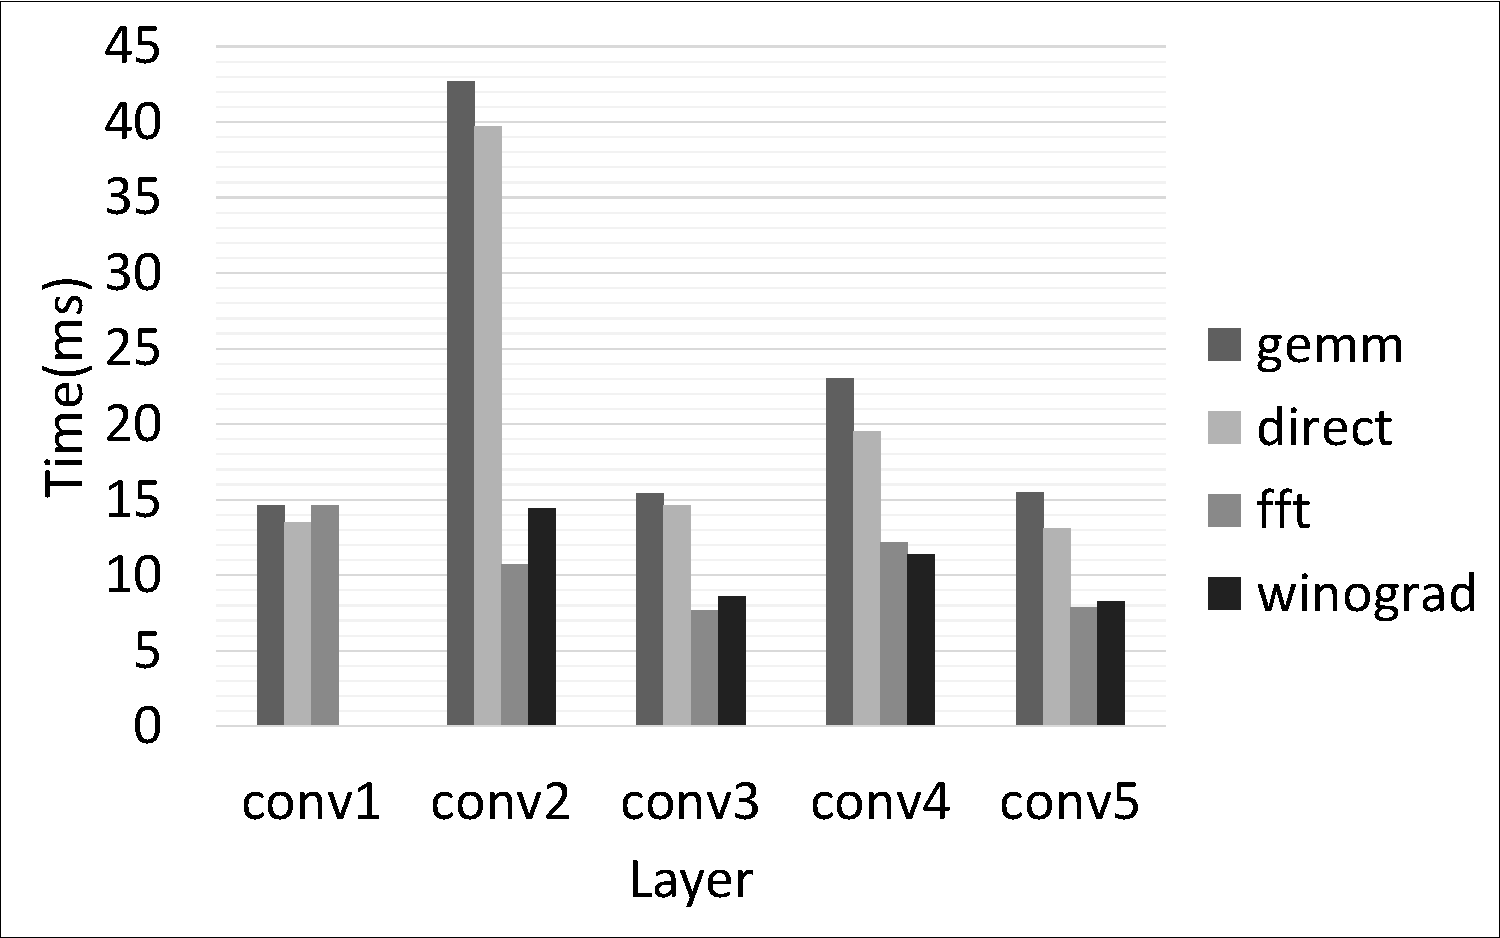
\includegraphics[width=.8\linewidth]{./figures/layerwise_fwd}
  \label{fig_layerwise_fwd}}

  \subfloat[The execution time by batch sizes] {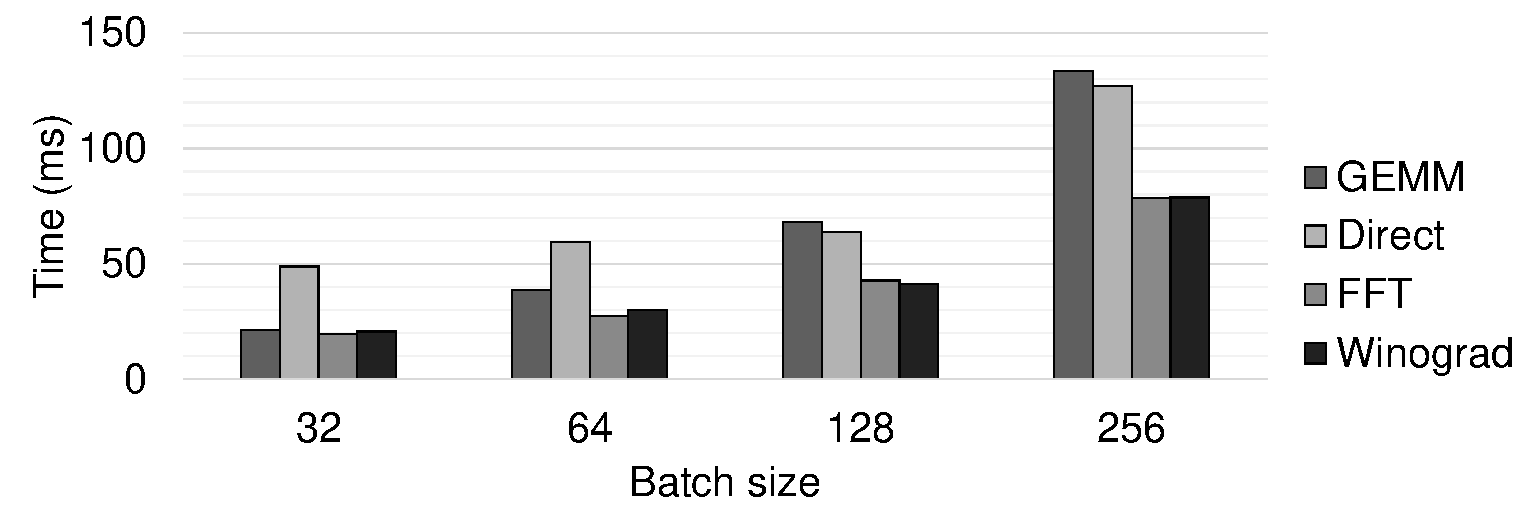
\includegraphics[width=.8\linewidth]{./figures/gpu_time_fwd}
  \label{fig_gpu_time_fwd}}


  \caption{The execution time of the forward computation.}
  \label{fig_layerwise}
\end{figure}

\begin{figure*}[htbp]
  \centering
  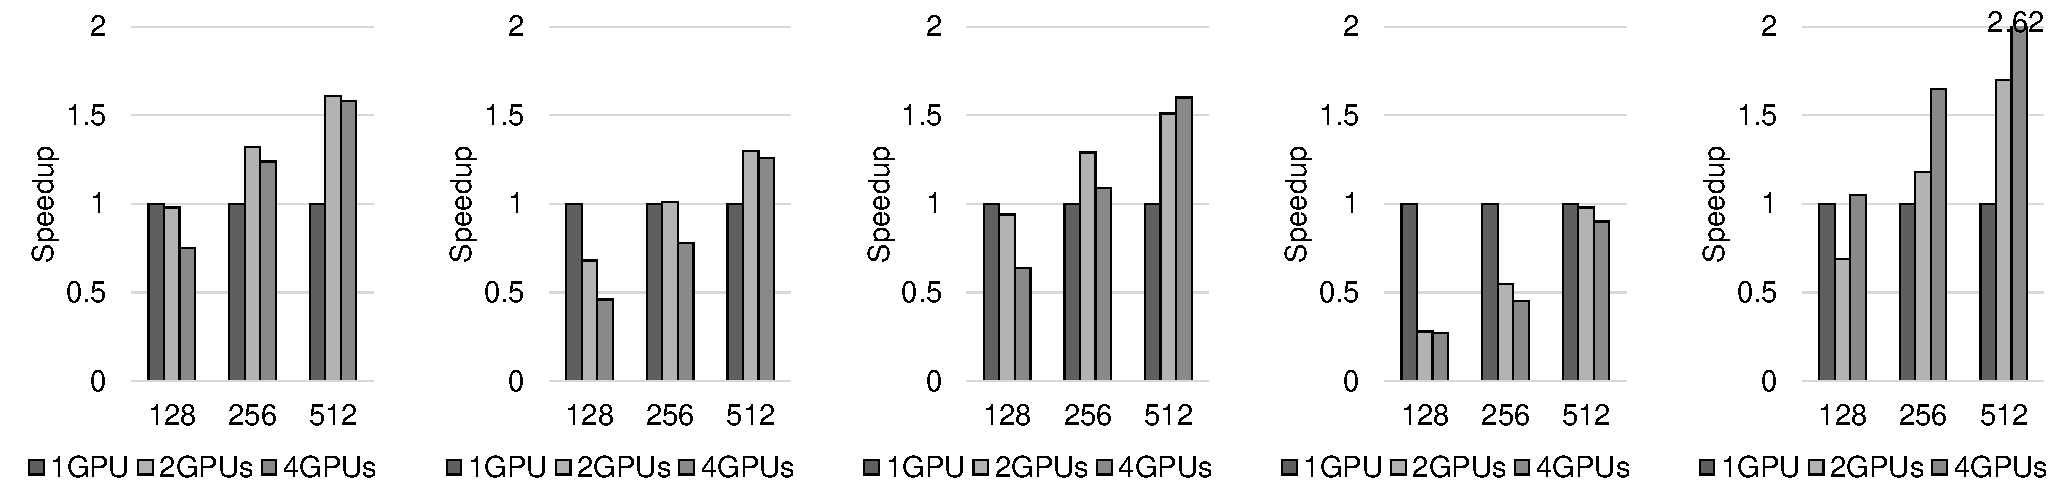
\includegraphics[width=.8\linewidth]{./figures/MG}
  \subfloat[Caffe]{\makebox[.19\linewidth][]{}}
  \subfloat[Torch]{\makebox[.19\linewidth][]{}}
  \subfloat[TensorFlow]{\makebox[.18\linewidth][]{}}
  \subfloat[CNTK]{\makebox[.18\linewidth][]{}}
  \subfloat[CNTK 1bit-SGD]{\makebox[.18\linewidth][]{}}
\caption{Speedup (over a single GPU) of multi-GPU training of the AlexNet models.}
\label{fig_mg}
\end{figure*}

 The result tells us that \textsf{FFT} is usually the fastest because of much less FP operation count (\textit{i.e.}, much less algorithm complexity). Especially, \textsf{FFT} is much faster than others in \textsf{conv2} with $5 \times 5$ convolution filter because the complexity of \textsf{FFT} does not depend on the filter size. \textsf{Winograd} also reduces FP operation count by more than a half. Thus, its performance is comparable to \textsf{FFT} in the layers with $3 \times 3$ convolution filters (\textsf{conv3}, \textsf{conv4}, and \textsf{conv5}).